\documentclass[10pt,fleqn]{article} % Default font size and left-justified equations
\usepackage[%
    pdftitle={Résolutions de problèmes de statique : PFS 2D},
    pdfauthor={Xavier Pessoles}]{hyperref}

\input{style/new_style}
\input{style/macros_SII}
\usepackage{multicol}
\usepackage{siunitx}
%\usepackage{picins}
 \fichetrue
%\fichefalse

\proftrue
\proffalse

\tdtrue
%\tdfalse

\courstrue
\coursfalse

\newif\ifnormal
\normaltrue
%\normalfalse

\newif\ifdifficile
\difficilefalse
%\difficiletrue

\newif\iftdifficile
\tdifficilefalse
%\tdifficiletrue

% -------------------------------------
% Déclaration des titres
% -------------------------------------

\def\discipline{Sciences \\Industrielles de \\ l'Ingénieur}
\def\xxtete{Sciences Industrielles de l'Ingénieur}


\def\classe{\textsf{PTSI$\star$ -- PT}}
\def\xxnumpartie{-- GE -- }
\def\xxpartie{Modéliser le comportement des systèmes électro mécaniques}

\def\xxnumchapitre{ }%Révision 1 \vspace{.2cm}}
\def\xxchapitre{\hspace{.12cm}}% Résolution des problèmes de statique -- Statique 2D}

\def\xxposongletx{2}
\def\xxposonglettext{1.45}
\def\xxposonglety{19}%16

\def\xxonglet{\textsf{-- GE -- }}

\def\xxactivite{TD}
\def\xxauteur{\textsl{Fabrice Sincère}}


\def\xxtitreexo{Exercices  \ifnormal $\star$ \else \fi \ifdifficile $\star\star$ \else \fi \iftdifficile $\star\star\star$ \else \fi}
\def\xxsourceexo{\hspace{.2cm} \footnotesize{Fabrice SINCERE}}

\def\xxcompetences{%
\textsl{%
\textbf{Savoirs et compétences :}\\} \vspace{-.5cm}
%\begin{itemize}
%\item \textit{Res2.C18} : principe fondamental de la statique:
%\item \textit{Res2.C19} : équilibre d’un solide, d’un ensemble de solides;
%\item \textit{Res2.C20} : théorème des actions réciproques.
%\end{itemize}
}

\def\xxfigures{
%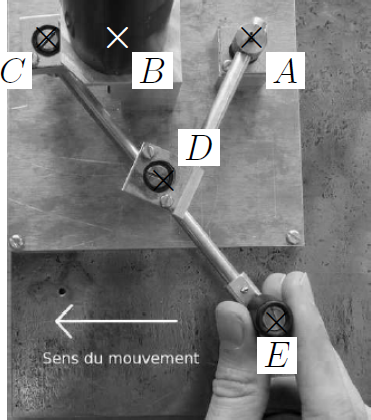
\includegraphics[width=.65\textwidth]{images/fig_00}
}%figues de la page de garde

\def\xxpied{%
Révision statique -- Résolution des problèmes de statique plane\\
Fiche 1 -- \xxactivite%
}

\setcounter{secnumdepth}{5}
%---------------------------------------------------------------------------

\usepackage{bm}
\begin{document}
%\chapterimage{png/Fond_Cin}
\input{style/new_pagegarde}
\vspace{4.5cm}
\pagestyle{fancy}
\thispagestyle{plain}


\def\columnseprulecolor{\color{ocre}}
\setlength{\columnseprule}{0.4pt} 

\ifprof
\begin{multicols}{2}
\else
\begin{multicols}{2}
\fi
\section*{MCC à excitation indépendante}


Une machine d'extraction est entraînée par un moteur à courant continu à excitation
indépendante.
L'inducteur est alimenté par une tension $u = \SI{600}{V}$ et parcouru par un courant d'excitation
d'intensité constante : $i = \SI{30}{A}$.
L'induit de résistance $R = \SI{12}{m \Omega}$ est alimenté par une source fournissant une tension $U$
réglable de $\SI{0}{V}$ à sa valeur nominale : $U_N = \SI{600}{V}$.
L'intensité $I$ du courant dans l'induit a une valeur nominale : $I_N = \SI{1,50}{kA}$.
La fréquence de rotation nominale est $n_N = \SI{30}{tr/min}$. 

\section*{Démarrage}

\subparagraph{}\textit{ En notant $\Omega$ la vitesse angulaire du rotor, la fem du moteur a pour expression : $E = K\Omega$ avec $\Omega$ en rad/s. Quelle est la valeur de $E$ à l'arrêt ($n = 0$) ? 
}
\ifprof
\begin{corrige}
\end{corrige}
\else
\fi

\subparagraph{}\textit{Dessiner le modèle équivalent de l'induit de ce moteur en indiquant sur le schéma les
flèches associées à $U$ et $I$.}
\ifprof
\begin{corrige}
\end{corrige}
\else
\fi
\subparagraph{}\textit{ Ecrire la relation entre $U$, $E$ et $I$ aux bornes de l'induit, en déduire la tension $U_d$ à
appliquer au démarrage pour que $I_d = 1,2 I_N$. }
\ifprof
\begin{corrige}
\end{corrige}
\else
\fi

\subparagraph{}\textit{Citer un système de commande de la vitesse de ce moteur. }
\ifprof
\begin{corrige}
\end{corrige}
\else
\fi

\section*{ Fonctionnement nominal au cours d'une remontée en charge}

\subparagraph{}\textit{Exprimer la puissance absorbée par l'induit du moteur et calculer sa valeur numérique.}
\ifprof
\begin{corrige}
\end{corrige}
\else
\fi

\subparagraph{}\textit{Exprimer la puissance totale absorbée par le moteur et calculer sa valeur numérique. }
\ifprof
\begin{corrige}
\end{corrige}
\else
\fi

\subparagraph{}\textit{Exprimer la puissance totale perdue par effet Joule et calculer sa valeur numérique. }
\ifprof
\begin{corrige}
\end{corrige}
\else
\fi

\subparagraph{}\textit{Sachant que les autres pertes valent \SI{27}{kW}, exprimer et calculer la puissance utile et le
rendement du moteur.}
\ifprof
\begin{corrige}
\end{corrige}
\else
\fi

\subparagraph{}\textit{Exprimer et calculer le couple utile $T_u$ et le couple
électromagnétique $T_{em}$.}
\ifprof
\begin{corrige}
\end{corrige}
\else
\fi



\section*{ Fonctionnement au cours d'une remontée à vide}


\subparagraph{}\textit{ Montrer que le couple électromagnétique $T_{em}$ de ce moteur est proportionnel
à l'intensité $I$ du courant dans l'induit : $T_{em} = KI$. }
\ifprof
\begin{corrige}
\end{corrige}
\else
\fi


On admet que dans le fonctionnement au cours d'une remontée à vide, le couple
électromagnétique a une valeur $T_{em}'$ égale à 10\% de sa valeur nominale et garde cette valeur
pendant toute la remontée. 

\subparagraph{}\textit{Calculer l'intensité $I'$ du courant dans l'induit pendant la remontée. }
\ifprof
\begin{corrige}
\end{corrige}
\else
\fi


\subparagraph{}\textit{La tension $U$ restant égale à $U_N$, exprimer puis calculer la fem $E'$ du moteur. }
\ifprof
\begin{corrige}
\end{corrige}
\else
\fi


\subparagraph{}\textit{ Exprimer, en fonction de $E'$, $I'$ et $T_{em}'$, la nouvelle fréquence de rotation $n'$. Calculer sa
valeur numérique. }
\ifprof
\begin{corrige}
\end{corrige}
\else
\fi



\newpage

\section*{Moteur à courant continu à aimants permanents (moteur de
rétroviseur électrique)}

\setcounter{exo}{0}

Un moteur de rétroviseur électrique d’automobile a les caractéristiques suivantes :
\begin{itemize}
\item moteur à courant continu à aimants permanents;
\item 62 grammes, $\Phi$ \SI{28}{mm} longueur \SI{38}{mm};
\item tension nominale $U_N=\SI{12}{V}$;
\item fem (E en V) = $10^{-3} \times$ vitesse de rotation (n en tr/min);
\item résistance de l’induit $R=\SI{3,5}{W}$;
\item pertes collectives \SI{1,6}{W}.
\end{itemize}
Le moteur est alimenté par une batterie de fem \SI{12}{V}, de
résistance interne négligeable (voir figure).

\begin{center}
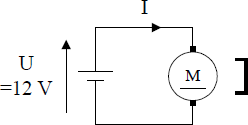
\includegraphics[width=.9\linewidth]{images/fig_01}
\end{center}

\subparagraph{}\textit{À vide, le moteur consomme \SI{0,20}{A}. Calculer sa fem et en déduire sa vitesse de rotation.}
\ifprof
\begin{corrige}
\end{corrige}
\else
\fi


\subparagraph{}\textit{Que se passe-t-il si on inverse le branchement du moteur ?}
\ifprof
\begin{corrige}
\end{corrige}
\else
\fi

En charge, au rendement maximal, le moteur consomme 0,83 A.
\subparagraph{}\textit{Calculer :
\begin{itemize}
\item la puissance absorbée;
\item les pertes Joule;
\item la puissance utile;
\item le rendement maximal;
\item la vitesse de rotation;
\item la puissance électromagnétique;
\item le couple électromagnétique;
\item le couple utile;
\item le couple des pertes collectives.
\end{itemize}}
\ifprof
\begin{corrige}
\end{corrige}
\else
\fi


\subparagraph{}\textit{Justifier que le couple électromagnétique est proportionnel au courant d’induit.
Vérifier que : $T_{em}(en Nm) = 9,55\times 10^{-3} \times I$ (en A).}
\ifprof
\begin{corrige}
\end{corrige}
\else
\fi



\subparagraph{}\textit{Calculer le courant au démarrage.
En déduire le couple électromagnétique de démarrage.}
\ifprof
\begin{corrige}
\end{corrige}
\else
\fi


\subparagraph{}\textit{Le moteur tourne sous tension nominale.
Que se passe-t-il si un problème mécanique provoque le blocage du rotor ?}
\ifprof
\begin{corrige}
\end{corrige}
\else
\fi

\newpage


\section*{Moteur à courant continu à excitation série}

\setcounter{exo}{0}

Un moteur à courant continu à excitation série est alimenté par une source de tension continue
et constante $U = \SI{220}{V}$.
Pour simplifier l’étude, nous négligerons les résistances de l’inducteur et de l’induit, ainsi que
les pertes collectives.

\subparagraph{}\textit{Montrer que le couple du moteur est proportionnel au carré du courant qu’il consomme.}
\ifprof
\begin{corrige}
\end{corrige}
\else
\fi

\subparagraph{}\textit{Montrer que le couple est inversement proportionnel au carré de la vitesse de rotation.}
\ifprof
\begin{corrige}
\end{corrige}
\else
\fi

\subparagraph{}\textit{En déduire que le moteur s’emballe à vide.}
On peut écrire que : $T_u = \dfrac{a}{n^2}$ avec 
\begin{itemize}
\item $T_u$ : couple utile du moteur (en Nm);
\item $n$ : vitesse de rotation (en tr/min);
\item $a$ : constante.
\end{itemize}
La plaque signalétique d’un moteur indique : \SI{220}{V} et $\SI{1200}{tr/min}$ et $\SI{6,8}{A}$.

\subparagraph{}\textit{En déduire la valeur numérique de la constante $a$.}
\ifprof
\begin{corrige}
\end{corrige}
\else
\fi

Par la suite, on prendra : $a = \SI{20e6}{Nm(tr/min)^2}$.



\subparagraph{}\textit{Tracer l’allure de la caractéristique mécanique $Tu(n)$.}
\ifprof
\begin{corrige}
\end{corrige}
\else
\fi

\subparagraph{}\textit{Le moteur entraîne un compresseur de couple résistant constant \SI{10}{Nm}.
En déduire la vitesse de rotation de l’ensemble.}
\ifprof
\begin{corrige}
\end{corrige}
\else
\fi

\subparagraph{}\textit{Le moteur entraîne un ventilateur dont le couple résistant est proportionnel au carré de la
vitesse de rotation (\SI{15}{Nm} à \SI{1000}{tr/min}).
En déduire la vitesse de rotation de l’ensemble.}



\newpage

\section*{Hacheur série}

\setcounter{exo}{0}

On alimente un moteur à courant continu dont le schéma équivalent est donné ci-dessous, à
l'aide d'un hacheur.
L'interrupteur électronique $K$ et la diode sont supposés parfaits.
La période de hachage est $T$, le rapport cyclique $\alpha$.
L'inductance $L$ du bobinage de l'induit du moteur a une valeur suffisante pour que la forme du
courant dans l'induit soit pratiquement continue.
Le hacheur est alimenté par une tension continue $E = \SI{220}{V}$.
La f.e.m. $E'$ du moteur est liée à sa vitesse de rotation $n$ par la relation :
$E' = 0,20 n$ avec $E'$ en $V$ et $n$ en tr/min. L'induit a pour résistance $R = \SI{2,0}{W}$.

\begin{center}
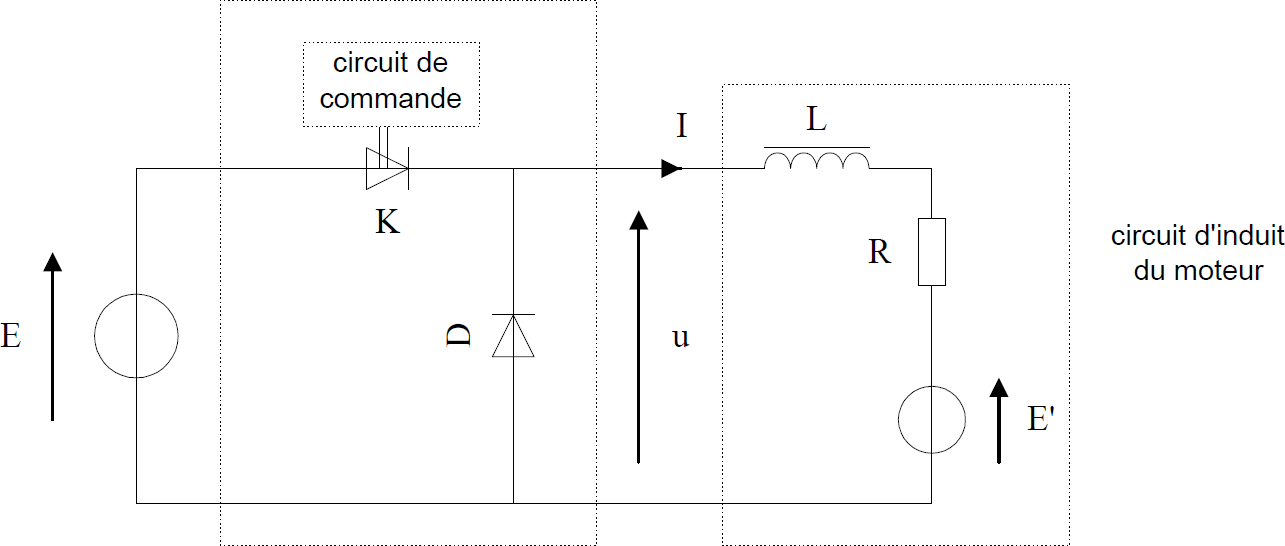
\includegraphics[width=\linewidth]{images/fig_03}
%\textit{}
\end{center}


\subsection*{Etude de la tension $u$ pour $\alpha = 0,80$}
\subparagraph{}\textit{Représenter, en la justifiant, l'allure de la tension $u$.
On prendra comme instant origine celui où l'interrupteur $K$ se ferme.}
\ifprof
\begin{corrige}
\end{corrige}
\else
\fi

\subparagraph{}\textit{Déterminer l'expression littérale de la valeur moyenne $< u >$ de la tension $u$, en fonction
de $E$ et du rapport cyclique $\alpha$. Calculer sa valeur numérique.}
\ifprof
\begin{corrige}
\end{corrige}
\else
\fi



\subsection*{Fonctionnement du moteur pour $\alpha = 0,80$}
\subparagraph{}\textit{Le moteur fonctionne en charge, la valeur moyenne du courant d'induit est $< I > = \SI{10}{A}$.
Déterminer $E'$ et en déduire $n$.}
\ifprof
\begin{corrige}
\end{corrige}
\else
\fi


Le dispositif de commande du hacheur est tel que le rapport cyclique a est proportionnel à
une tension de commande $u_C$ : $\alpha = 100\%$ pour $u_C =\SI{5}{V}$.

\subparagraph{}\textit{Tracer la caractéristique $< u >$ en fonction de $u_C$.}



\newpage

\section*{Hacheur série}

\setcounter{exo}{0}
Un moteur à courant continu travaillant à couple constant est inclus dans le montage ci-dessous.


\begin{center}
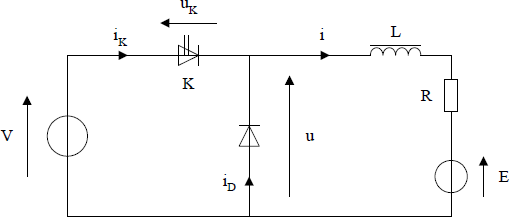
\includegraphics[width=\linewidth]{images/fig_04}
%\textit{}
\end{center}


Le hacheur fonctionne à une fréquence $f = \SI{500}{Hz}$.
L’interrupteur $K$ est fermé lorsque $0 < t < \alpha T$ et ouvert entre $\alpha T$ et $T$.
La diode est supposée parfaite.
L'inductance de la bobine de lissage $L$ est de valeur suffisante pour que le courant dans le
moteur soit considéré comme constant : $i= I = \text{cte}$.
La résistance de l’induit du moteur est : $R = \SI{1}{\Omega}$.

\subparagraph{}\textit{ Représenter les allures de $u$ et $u_K$ en fonction du temps.}
\subparagraph{}\textit{ Exprimer la valeur moyenne de $u$ en fonction de $V$ et $\alpha$.}
\subparagraph{}\textit{ Représenter les allures de $i_K$ et $i_D$ en fonction du temps.}
\subparagraph{}\textit{ Exprimer les valeurs moyennes des courants $i_K$ et $i_D$ en fonction de $I$ et $\alpha$.}
\subparagraph{}\textit{ Déterminer l'intensité $I$ du courant dans le moteur en fonction de $V$, $E$, $R$ et $\alpha$.}

\subparagraph{}\textit{ Application numérique : calculer $< u >$, $I$ et $< i_D >$ pour $V = \SI{220}{V}$, $E = \SI{145}{V}$ et $\alpha = 0,7$.}

\subparagraph{}\textit{ Établir la relation liant la vitesse $n$ du moteur (en tr/min) à $\alpha$ pour $E = 0,153 n$, sachant que $R = \SI{1}{W}$, $V = \SI{220}{V}$ et $I =\SI{9}{A}$.}
\subparagraph{}\textit{ Tracer $n$ en fonction de $\alpha$.}

\newpage

\section*{Hacheur parallèle}
\setcounter{exo}{0}

\begin{center}
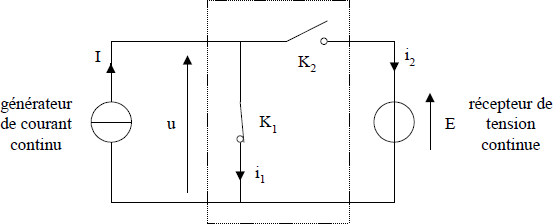
\includegraphics[width=\linewidth]{images/fig_05}
%\textit{}
\end{center}
Les deux interrupteurs électroniques sont supposés parfaits.


\subparagraph{}\textit{On donne les séquences de conduction de $K_1$ et $K_2$. Compléter les chronogrammes.}
\ifprof
\begin{corrige}
\end{corrige}
\else
\fi

\begin{center}
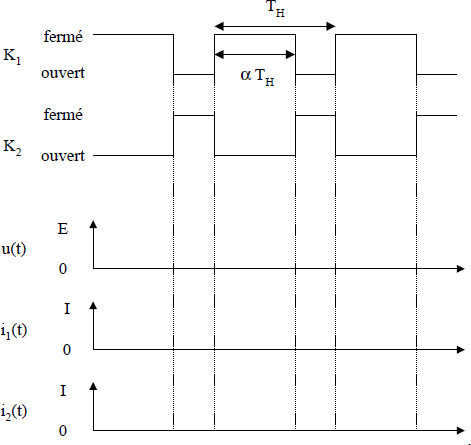
\includegraphics[width=\linewidth]{images/fig_06}
%\textit{}
\end{center}

\subparagraph{}\textit{Donner la relation entre $< u >$, $\alpha$ et $E$.}


\ifprof
\end{multicols}
\else
\end{multicols}
\fi


\end{document}

\subparagraph{}\textit{}
\ifprof
\begin{corrige}
\end{corrige}
\else
\fi

\begin{center}
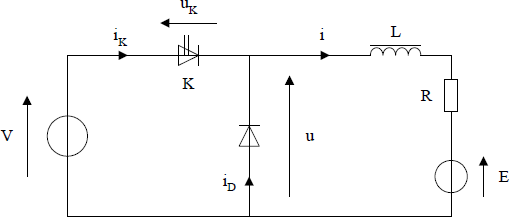
\includegraphics[width=\linewidth]{images/fig_04}
%\textit{}
\end{center}

